
\chapter{连续介质力学}\label{chap2}

这是第二章,目的是展示一些示例

\section{欧拉视角下的动力学}

\subsection{图片示例}

附上照片一张,来源 Wikipedia。

\begin{figure}[htbp]
  \centering
  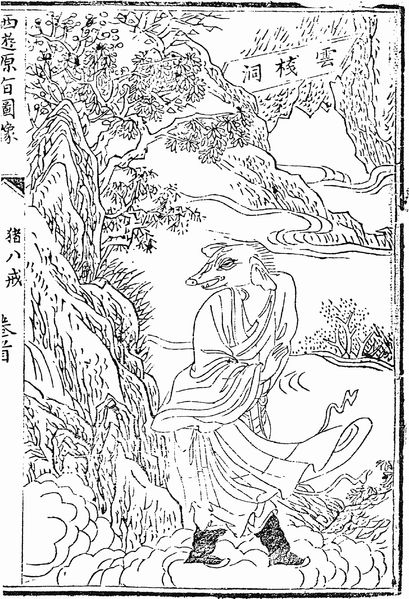
\includegraphics[scale=0.5]{./images/zhubajie.png}
  \caption{这是一张图}
  \label{fig:example}
\end{figure}

\subsection{表格示例}
\begin{table}[htb]
  \centering
  \caption{模板中的表格宏包}
  \label{tab:simple-table}
    \begin{tabular}{ll}
      \toprule
      \multicolumn{1}{m{20mm}}{\heiti\centering 宏包} & \multicolumn{1}{m{80mm}}{\heiti\centering 描述} \\
      \midrule
      longtable & 绘制跨页的表格。 \\
      booktabs & 三线表中的那三条线的命令来自这里。\\
      caption2 & 用于设置标题很方便,已经 obsolated,不过 \TeX Live 中还有。\\
      multirow & 跨行的单元格用这个宏包。\\
      dcolumn  & 想让表格小数点对齐吗?用这个宏包吧。\\
      \rowcolor[gray]{.9} colortbl & 表格上色。自己看着爽而已,打印出来都是黑白的。 \\
      threeparttable & 用来给表格添加脚注啥的很方便。 \\
      array & 忘了用来做什么了,但似乎很重要。 \\
      \bottomrule
    \end{tabular}
\end{table}

\subsection{定理示例}

可以到zjuthesis.cls里的定理环境设置模块里看看有什么需要的定理。

\begin{defn}
子曰:「道千乘之国,敬事而信,节用而爱人,使民以时。」
\end{defn}

\begin{thm}
犯我强汉者,虽远必诛。\hfill —— 陈汤(汉)
\end{thm}

\begin{pro}
  以下是证明1.
\end{pro}

\begin{pro*}
  以下是证明2.
\end{pro*}

\begin{prop}
天不言自高,水不言自流。
\begin{gather*}
\begin{split} 
\varphi(x,z)
&=z-\gamma_{10}x-\gamma_{mn}x^mz^n\\
&=z-Mr^{-1}x-Mr^{-(m+n)}x^mz^n
\end{split}\\[6pt]
\begin{align} \zeta^0&=(\xi^0)^2,\\
\zeta^1 &=\xi^0\xi^1,\\
\zeta^2 &=(\xi^1)^2,
\end{align}
\end{gather*}
\end{prop}

\subsection{算法示例}

大家有时候还需要写一些算法的伪代码,模板里面已经有支持了,看看算法\ref{alg:put-into-refri},具体的实用还需要参考CTAN上的关于{\textsf{algorithmicx}}宏包的文档,包括自定义关键字等等。

\begin{algorithm}
\caption{把猪八戒放进冰箱}
\label{alg:put-into-refri}
\begin{algorithmic}[1]
\Require N头动物,不知道是不是猪八戒  \Comment{我是注释} 
\Ensure 你造吗,这个程序木有输出,想怎样?
\State 先热热身:)
\For{$i=1,\dots ,N$} \Comment{我是个For循环}
\If {是猪八戒}
	\State 打开冰箱门,把第$i$个放进冰箱,关上冰箱门
\Else 
	\State 下一个
\EndIf
\EndFor
\end{algorithmic}
\end{algorithm}

\subsection{公式示例}

贝叶斯公式如式 (\ref{equ:chap1:bayes}),其中 $p(y|\mathbf{x})$ 为后验;$p(\mathbf{x})$ 为先验;分母 $p(\mathbf{x})$ 为归一化因子。

\begin{equation}
\label{equ:chap1:bayes}
p(y|\mathbf{x}) = \frac{p(\mathbf{x},y)}{p(\mathbf{x})}=
\frac{p(\mathbf{x}|y)p(y)}{p(\mathbf{x})} 
\end{equation}

论文里面公式越多,\TeX 就越 happy。再看一个 \textsf{amsmath} 的例子:

\newcommand{\envert}[1]{\left\lvert#1\right\rvert} 

\begin{equation}\label{detK2}
\det\mathbf{K}(t=1,t_1,\dots,t_n)=\sum_{I\in\mathbf{n}}(-1)^{\envert{I}}
\prod_{i\in I}t_i\prod_{j\in I}(D_j+\lambda_jt_j)\det\mathbf{A}
^{(\lambda)}(\overline{I}|\overline{I})=0.
\end{equation} 

大家在写公式的时候一定要好好看 \textsf{amsmath} 的文档,并参考模板中的用法:

\begin{multline*}\tag{[b]} % 这个出现在索引中的
\int_a^b\biggl\{\int_a^b[f(x)^2g(y)^2+f(y)^2g(x)^2]
 -2f(x)g(x)f(y)g(y)\,dx\biggr\}\,dy \\
 =\int_a^b\biggl\{g(y)^2\int_a^bf^2+f(y)^2
  \int_a^b g^2-2f(y)g(y)\int_a^b fg\biggr\}\,dy
\end{multline*}

其实还可以看看这个多级规划:

\begin{equation}\label{bilevel}
\left\{\begin{array}{l}
\max\limits_{{\mbox{\footnotesize\boldmath $x$}}} F(x,y_1^*,y_2^*,\cdots,y_m^*)\\[0.2cm]
\mbox{subject to:}\\[0.1cm]
\qquad G(x)\le 0\\[0.1cm]
\qquad(y_1^*,y_2^*,\cdots,y_m^*)\mbox{ solves problems }(i=1,2,\cdots,m)\\[0.1cm]
\qquad\left\{\begin{array}{l}
    \max\limits_{{\mbox{\footnotesize\boldmath $y_i$}}}f_i(x,y_1,y_2,\cdots,y_m)\\[0.2cm]
    \mbox{subject to:}\\[0.1cm]
    \qquad g_i(x,y_1,y_2,\cdots,y_m)\le 0.
    \end{array}\right.
\end{array}\right.
\end{equation}


